\section{Konzept}

Lorem ipsum

\subsection{Migration Benachrichtigungen}

Mit IP5 wurde bereits ein Client umgesetzt.
Dieser muss für IP6 migiert werden.

Architektur Anbindung Rest \\
Architektur Anbindung Firebase \\

\clearpage


\subsection{Integration Text To Speech}

\subsubsection*{Benutzeroberfläche}

Erweiterung Inbox um T2S Icon. \\
Erweiterung Admin UI um Checkbox. \\
Zusätzlich Configuration Page mit preferences. \\

\subsubsection*{Konfiguration}
Erweiterung NotificationType um ein boolean Flag für isTextToSpeech.
Wenn Aktiviert, wird Benachrichtigung bei Empfang vorgelesen.
Text To Speech kann auf Client Seite dekativiert werden.
Ist es deaktiviert, werden keine Benachrichtigungen vorgelesen.
Audio Signal, dass Benachrichtung empfangen wurde ertönt aber trotzdem.
Keine zusätzlichen Endpoints am Cloud Service nötig. \\


\subsection*{Laufzeitsicht}

Empfang und Versenden gleich wie bei IP5.
Benachrichtigung enthält zudem neu Flag ob T2S gebraucht werden soll.
Wenn ja, wird Vorlesen an T2S Service delegiert.

\begin{figure}[h]
    \centering
    \begin{minipage}[b]{0.9\textwidth}
        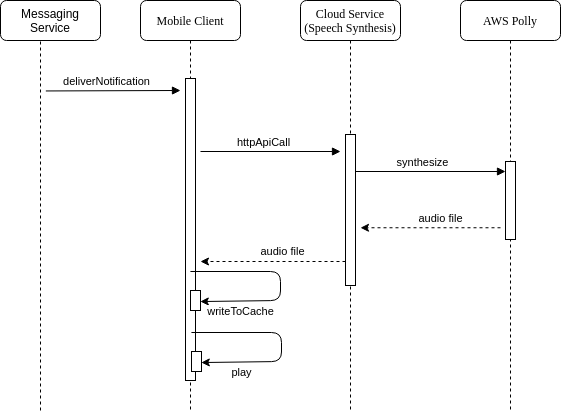
\includegraphics[width=\textwidth]{graphics/diagramms/Sequence_Speech_Synth_V01}
        \caption{Ablauf Benachrichtigung empfangen}
    \end{minipage}
\end{figure}

\clearpage

\subsection{Integration Gegensprechanlage}

\subsubsection*{Benutzeroberfläche}

Button Screen wie IP5 \\
Active Call Screen \\
Erweiterte Inbox \\
Neue Screens für Gegensprechanlage. \\
Erweiterung Admin UI für Konfiguration CallType \\


\subsubsection*{Konfiguration}
Erweiterung Configuration Domain um CallType.
Hat text property, dass als Anzeige auf dem Button dient.
Hat Liste von Clients, die im Call angesprochen werden können.

\subsubsection*{Laufzeitsicht}

\begin{figure}[h]
    \centering
    \begin{minipage}[b]{0.9\textwidth}
        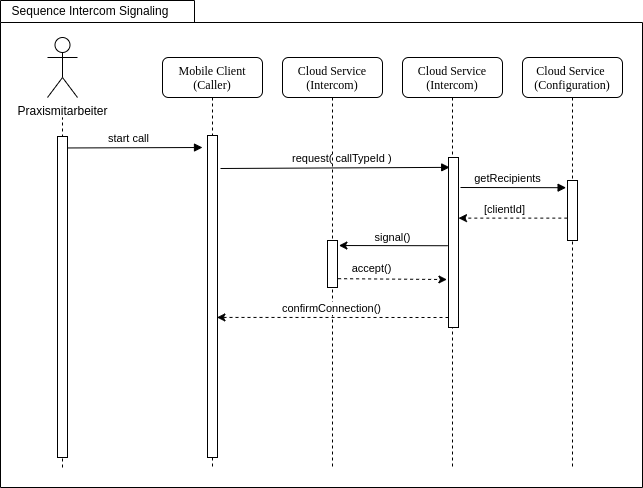
\includegraphics[width=\textwidth]{graphics/diagramms/Sequence_Intercom_Broking_V01}
        \caption{Ablauf Verbindungsaufbau Gegensprechanalge}
    \end{minipage}
\end{figure}

\clearpage

\subsection{Übersicht Erweiterung Praxisruf Cloud Service}

<< Erweitertes ERD für Configuration Domain (Cloud Service) >>

\clearpage
